
\subsection{Desired properties of a chemistry benchmark} \label{sec:desired-properties}

\begin{itemize}
    \item \emph{End-to-end automation}. For model development, the evaluations must be run many times (e.g., on regular intervals of a training run).
    Approaches that rely on humans scoring the answers of a system\autocite{Schulze_Balhorn_2024, ai4science2023impact, castro2023large} can thus not be used.
    \item \emph{Careful validation by experts}. Manual curation is needed to minimize the number of incorrect or unanswerable questions.\autocite{northcutt2021pervasive}
    This is motivated by the observation that many widely used benchmarks are plagued by noisiness.\autocite{Frye_2023, Awg}
    \item \emph{Usable with models that support special treatment of molecules}. Some models, such as Galactica\autocite{taylor2022galactica}, use special tokenization or encoding procedures for molecules or equations.
    The benchmark system must encode the semantic meaning of various parts of the question or answer to support this.
    \item \emph{Usable with black box systems}. Many relevant systems do not provide access to model weights or raw logits.
    This might be the case because the systems are proprietary or because they involve not only \glspl{llm} but also external tools such as search \glspl{api} or code executors.\autocite{schick2024toolformer, karpas2022mrkl, yao2022react}
    Thus, a benchmark should not assume access to the raw model outputs but be able to operate on text completions.
    \item \emph{Probing capabilities beyond answering of \glspl{mcq}}. In real-world chemistry, as well as higher-level university education, multiple-choice questions are seldom utilized.
    Yet, most benchmarking frameworks focus on the \gls{mcq} setting because of the ease of evaluation. Realistic evaluations must measure capabilities beyond answering \gls{mcq}.
    \item \emph{Cover a diverse set of topics}. Chemistry, as the \enquote{central science}, bridges multiple disciplines.\autocite{Aspuru_Guzik_2018} To even just approximate \enquote{chemistry capabilities} the topics covered by a chemistry benchmark must be very diverse.
    \item \emph{Cover diverse skills}. To holistically judge performance it is important to cover questions relying on reasoning, calculation, knowledge, intuition.
    \item \emph{Cover a range of difficulty levels}. To allow for a continuous measure of improvement for a range of different (evolving) systems, a benchmark should cover a wide range of difficulty levels.
    \item \emph{Impossible to completely solve with current models}. A benchmark should contain questions that are impossible to solve with current models. If current models can solve all questions, the benchmark provides no useful signal.
\end{itemize}

\subsection{Related work}
Existing benchmarks such as those from \textcite{guo2023large}, \textcite{sun2023scieval}, \textcite{Schulze_Balhorn_2024}, \textcite{Cai_2024} fail to comply with most of the requirements stipulated above.
While these benchmarks could provide valuable insights in the short term, they cannot follow the rapid additions to the \gls{llm} space.
\chembench aims to correct this through a set of developments: compatibility with BigBench, end-to-end automation, a particular focus on chemical safety, employment of diverse prompting strategies, and specialized notation for molecules and mathematical symbols.
Moreover, our robust framework, including the platform \url{chembench.org}, will engage the community in open-source contributions.

\clearpage
\subsection{Benchmark corpus}
To ensure maximal interoperability with existing benchmarks or tools, we curated the data in an extended form of the widely used BigBench format.\autocite{srivastava2022beyond}
This also implies that future baselines can be built on top of our infrastructure if saved in the same format.

\Cref{fig:cb_humanset} shows the distribution of topics and required skills in the human subset of the \chembench corpus.

\begin{figure}
    \centering
    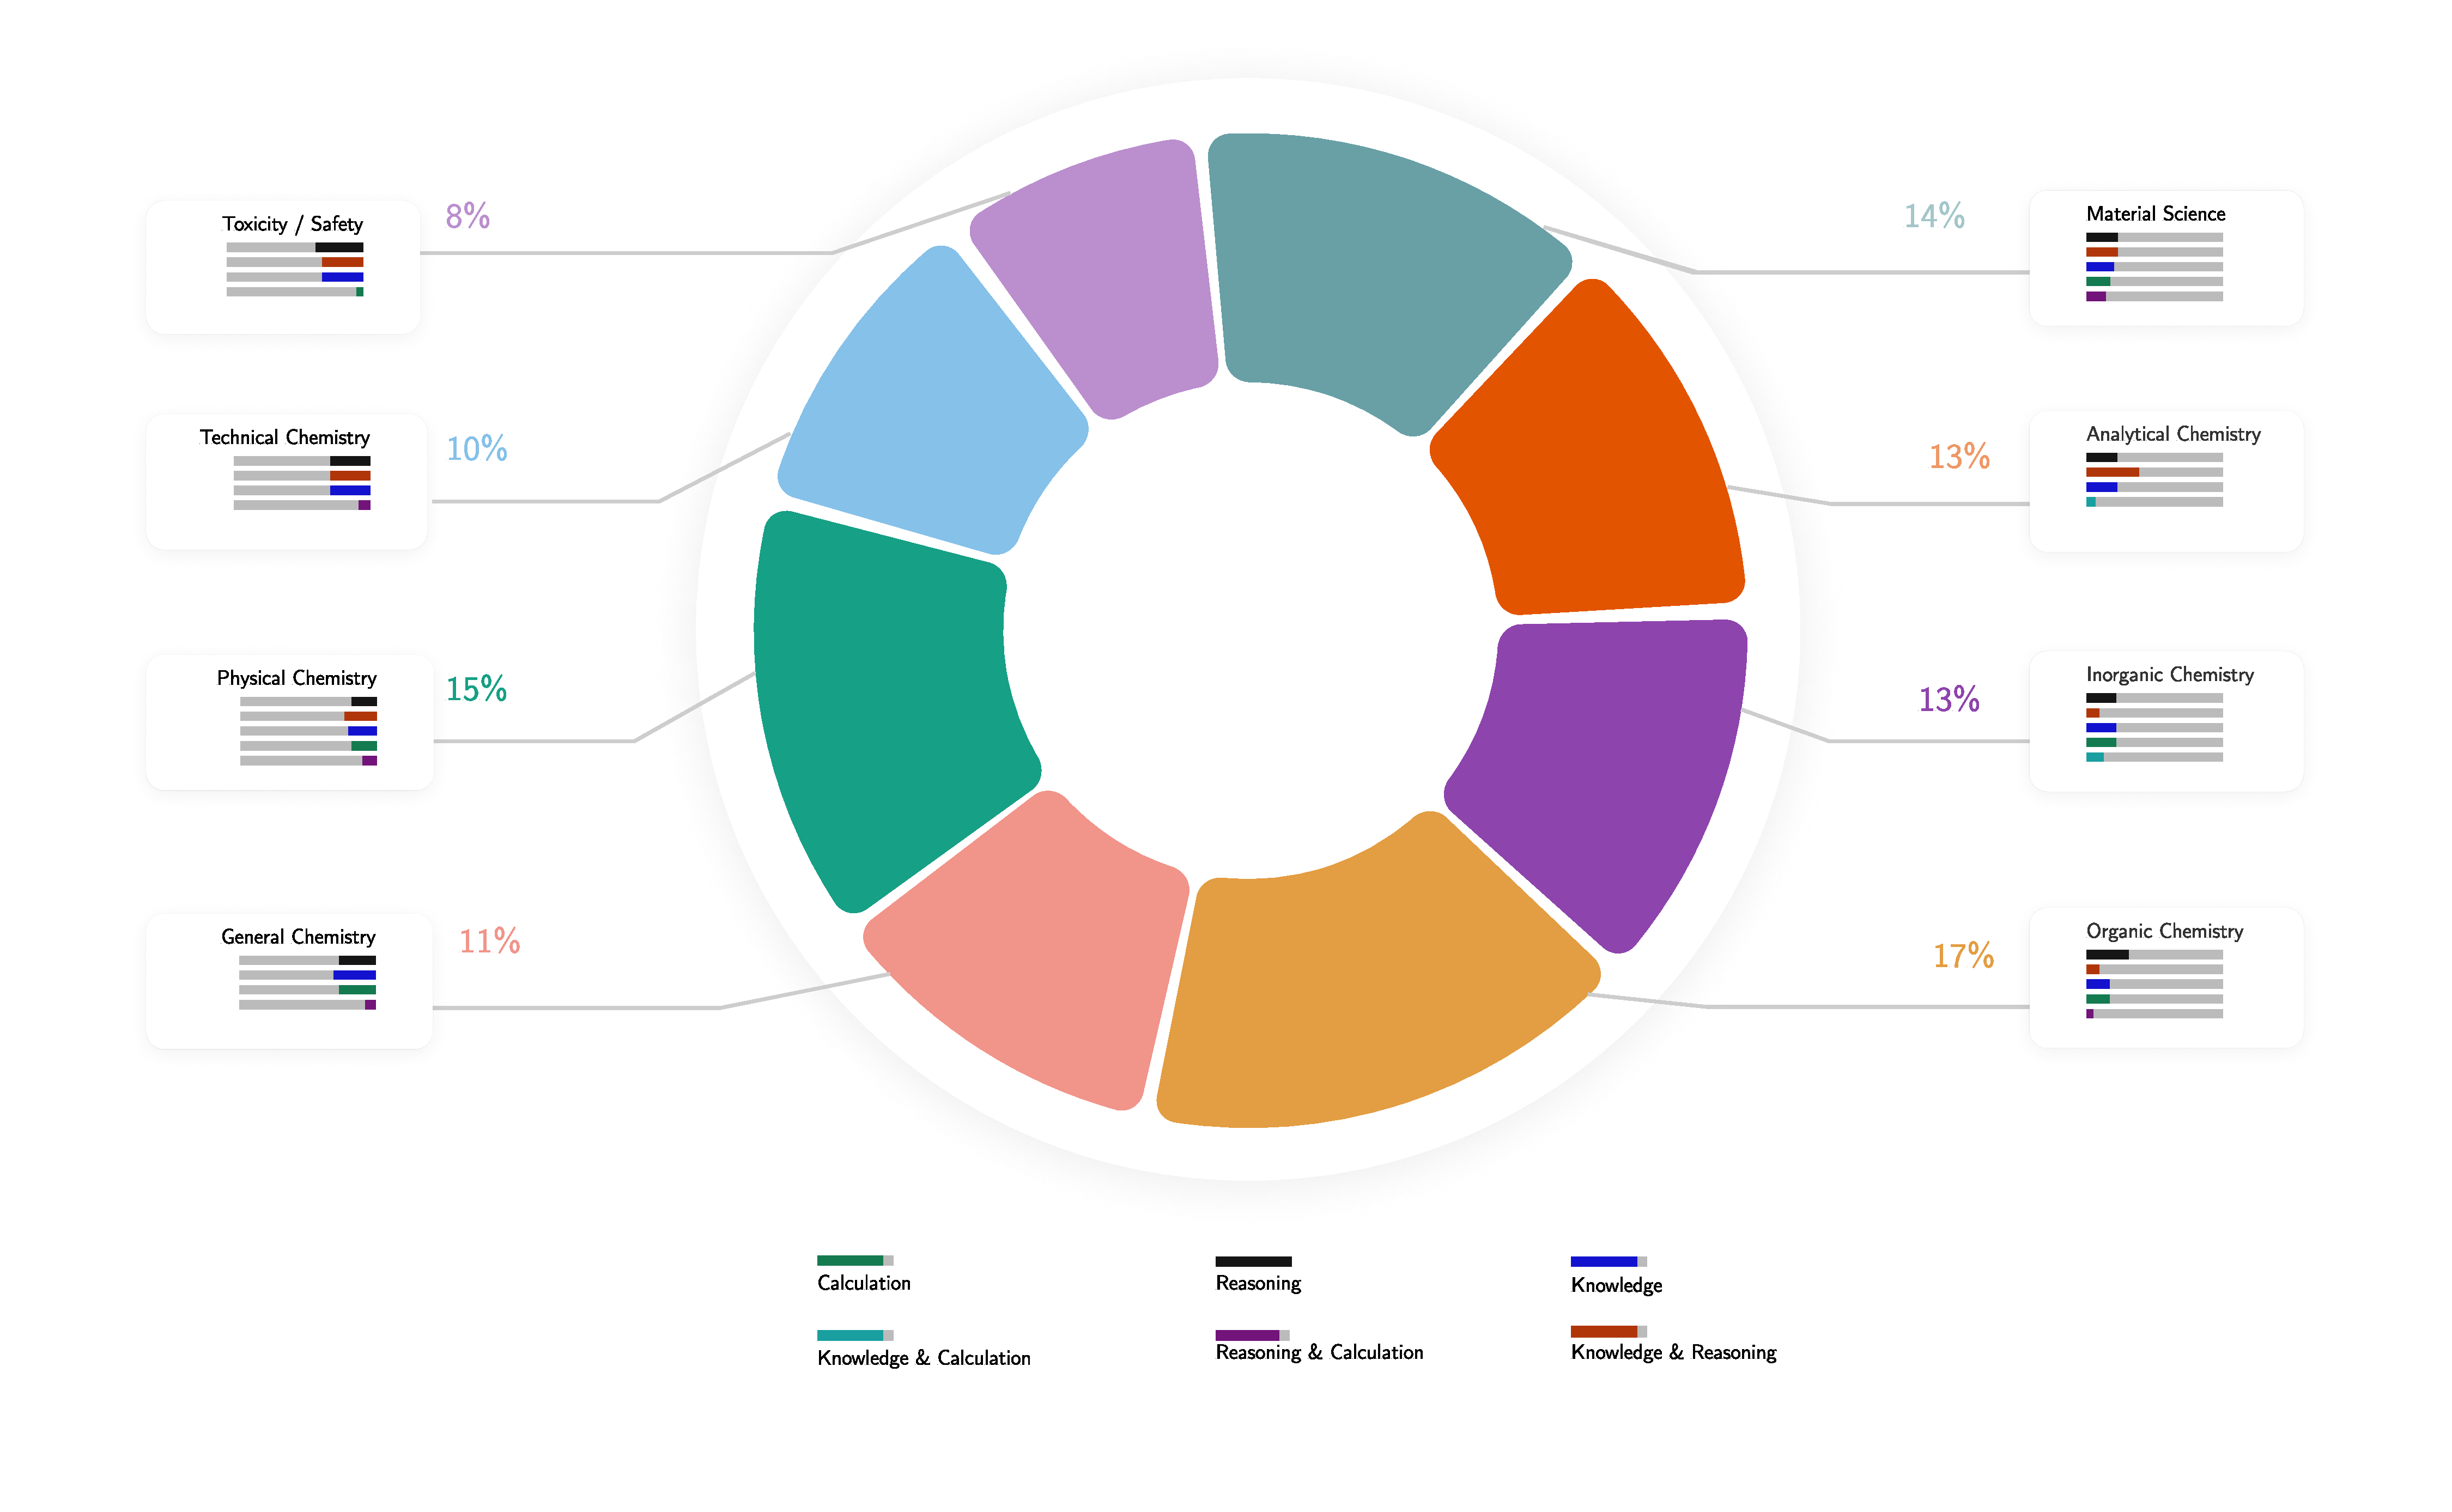
\includegraphics[width=\textwidth]{figures/cb_humanset_v3.pdf}
    \caption{\textbf{Composition of the human subset.} The circular plot shows the distribution of topics and required skills in the human subset of the \chembench corpus. The human subset is a representative subset of the full corpus, with a balanced distribution of topics and skills.}
    \label{fig:cb_humanset}
\end{figure}

%\Cref{fig:flesch_kincaid_reading_ease} shows the distribution of the Flesch-Kincaid reading ease scores of the questions.
%We see that the questions are generally complex to read.

% \begin{figure}[htb]
%     \centering
%     \includegraphics{figures/flesch_kincaid_reading_ease.pdf}
%     \caption{\textbf{Distribution of Flesch-Kincaid reading ease scores of the questions.} The Flesch-Kincaid reading ease score\autocite{flesch1948new} measures how easy a text is to read. It is calculated based on the average number of syllables per word and words per sentence. The higher the score, the easier the text is to read. The distribution of the questions' scores is shown in the histogram. }
%     \label{fig:flesch_kincaid_reading_ease}
%     \script{wordcloud.py}
% \end{figure}

\Cref{fig:question_count_barplot_mcq_vs_general} shows that most questions in our corpus are \gls{mcq}.
A substantial fraction, in contrast to other benchmarks, is open-ended.
% \begin{figure}[htb]
%     \centering
%     \includegraphics{figures/question_count_barplot_mcq_vs_general.pdf}
%     \caption{\textbf{Number of multiple choice questions vs.\ open-ended questions per topic.} The bar plot shows the number of \gls{mcq} and general questions per topic.}
%     \label{fig:question_count_barplot_mcq_vs_general}
%     \script{plot_statistics.py}
% \end{figure}

The corpus of the questions in \chembench, as shown in \Cref{tab:chembench_corpus_topic}, can be divided according to which chemical topic they belong to.

\begin{xltabular}{\textwidth}{p{2.7cm}p{4em}X}
        \caption{\textbf{Examples for each of the topics considered in the evaluation of the \chembench corpus.} The table shows the percentage of questions in the corpus that belong to each topic, as well as example questions.} \\

        \toprule
        Question Type & \% & Example Questions  \\
        \midrule
        Chemical Preference & 35.0 & Imagine an early virtual screening campaign setting (accounting for simple aspects such as oral availability and small molecular profile, but no other modalities such as covalency or bifunctionality). Which of the following two candidates would you prefer for further development? \\
        & & A. [START\_SMILES]N\#Cc1ccc(OCCCN2CC3CN(CCNS(=O)(=O)c4ccc(F)cc4)CC(C2)O3)cc1[END\_SMILES] \\
        & & B. [START\_SMILES]O=C1CC(c2ccc(CC(NS(=O)(=O)c3cc(Cl)cc(Cl)c3)c3nc4ccccc4[nH]3)cc2)S(=O)(=O)N1[END\_SMILES] \\
        \midrule
        Technical Chemistry & 1.5 & Which of the following statements is true about the different types of ideal reactors? \\
        & & A. In a batch reactor, the composition is uniformly mixed and remains the same throughout the reactor and at the exit \\
        & & B. In a batch reactor, the fluid passes through the reactor with no mixing of earlier and later entering fluid \\
        & & C. In a mixed flow reactor, the composition changes with time but is uniform everywhere within the reactor \\
        & & D. In a plug flow reactor, the fluid moves in single flow through the reactor with no mixing and no overtaking \\
        \midrule
        Organic Chemistry & 15.5 & What is the reaction mechanism that describes the following reaction (represented using reaction SMILES) [START\_RXNSMILES]CCCl.CO[Na]>>[Na]Cl.CCOC[END\_RXNSMILES]? \\
        & & A. $E_1$ \\
        & & B. $E_{cb}$ \\
        & & C. $S_N1$ \\
        & & D. $S_N2$ \\
        \midrule
        Toxicity/Safety & 24.2 & Pindolol and propranolol are (relatively nonselective) antagonists at $\beta_1$- and $\beta_2$-adrenoceptors. However, pindolol is a partial agonist, whereas propranolol is a pure antagonist. What follows from this? \\
        & & A. Pindolol has a greater therapeutic range than propranolol \\
        & & B. Pindolol has a longer half-life than propranolol \\
        & & C. Pindolol has intrinsic activity \\
        & & D. Pindolol is more lipophilic than propranolol \\
        & & E. Pindolol is more potent than propranolol \\
        \midrule
        Analytical Chemistry & 5.8 & Which of the following analytical methods is most appropriate for performing a survey analysis of a solid sample containing various metals? \\
        & & A. X-ray fluorescence analysis \\
        & & B. Differential pulse polarography \\
        & & C. Flame-atomic absorption spectroscopy \\
        & & D. Gas chromatography with flame ionization detector \\
        & & E. Hydride generation atomic absorption spectroscopy \\
        \midrule
        Materials Science & 3.1 & For NMR analysis, you need to digest the MOF in a strong acid to remove the linker and leave the metal clusters intact. Why would one choose \ce{HF} over \ce{HCl} for this purpose? \\
        & & A. \ce{F-} forms a stable bonds to the metal ions \\
        & & B. \ce{HF} has a better water solubility than \ce{HCl} \\
        & & C. \ce{HF} has a higher boiling point than \ce{HCl} \\
        & & D. \ce{HF} is a weaker acid than \ce{HCl} \\
        \midrule
        General Chemistry & 5.3 & Which of the following salts is an acidic salt? \\
        & & A. \ce{NH4Cl} \\
        & & B. \ce{Na2CO3} \\
        & & C. \ce{NaH2PO4} \\
        & & D. \ce{Zn(OH)Cl} \\
        \midrule
        Physical Chemistry & 6.3 & The Born-Oppenheimer (BO) approximation is widely used in computational chemistry, but its accuracy can vary depending on the system. Among the following options, for which system is the Born-Oppenheimer approximation likely to be least applicable? \\
        & & A. \ce{C60} \\
        & & B. \ce{CH4} \\
        & & C. \ce{Fe(CO)5} \\
        & & D. \ce{H2+} \\
        & & E. \ce{NaCl} \\
        \midrule
        Inorganic Chemistry & 3.3 & What is the oxidation number of the metal in the compound \ce{[ZrF7]^{3-}}\\
    \label{tab:chembench_corpus_topic}
\end{xltabular}

\normalsize

In addition, as shown in \Cref{tab:chembench_corpus_cognitive} the \chembench corpus can be divided considering the different skills needed to solve the questions.

\begin{xltabular}{\textwidth}{p{2.7cm}p{4em}X}
        \caption{\textbf{Examples for each of the required skills considered in the \chembench corpus.} The table shows the number of questions for each skill and an example question.} \\

        \toprule
        Required Skills & Number of Questions & Example Question \\
        \midrule
        Knowledge & 770 & Which of the following salts is an acidic salt? \\
        & & A. \ce{NH4Cl} \\
        & & B. \ce{Na2CO3} \\
        & & C. \ce{NaH2PO4} \\
        & & D. \ce{Zn(OH)Cl} \\
        \midrule
        Reasoning & 825 & How can the optical impact of quantum confinement on the electronic structure of a quantum dot be observed experimentally? \\
        & & A. By measuring atomic force microscopy \\
        & & B. By measuring fourier transform infrared spectroscopy \\
        & & C. By measuring photoluminescence spectrum \\
        & & D. By measuring the absorption spectroscopy \\
        \midrule
        Intuition & 1001 & Imagine an early virtual screening campaign setting (accounting for simple aspects such as oral availability and small molecular profile, but no other modalities such as covalency or bifunctionality). Which of the following two candidates would you prefer for further development? \\
        & & A. [START\_SMILES]CC1(C)Oc2ccc([N+](=O)[O-])cc2[C@@H](N2CCOCC2)[C\@\@H]1O[END\_SMILES] \\
        & & B. [START\_SMILES]Cc1ccccc1N=C(S)N1CCC(NC(=O)c2ccco2)CC1[END\_SMILES] \\
        \midrule
        Calculation & 91 & Given that the average molar mass of the polymer chains in this sample of poly(lactic acid) (PLA) is \SI{595}{g mol^{-1}} using end-group analysis, where \SI{0.1619}{g} of PLA was dissolved in \SI{25}{cm^3} of benzyl alcohol and titrated with \SI{0.0400}{mol dm^{-3}} \ce{KOH} solution. The volume of \ce{KOH} solution required to reach the endpoint was \SI{6.81}{cm^3}. What is the average number of monomer units in each polymer chain of this sample? \\
        \bottomrule

    \label{tab:chembench_corpus_cognitive}
\end{xltabular}

\normalsize


\clearpage
\subsection{Model performance}
We also evaluated the model performance on the entire \chembench corpus.
\Cref{fig:barplot_all_correct_all_questions} shows the fraction of questions that were answered correctly by the models.
Note that this ranking differs from the one on the \enquote{tiny} subset

\begin{figure}[htb]
    \centering
    \includegraphics{figures/overall_performance.pdf}
    \caption{\textbf{Overall performance of the models on the \chembench corpus.} The bar plot shows the fraction of questions that were answered completely correctly by the models. Scores computed on the entire \chembench corpus.}
    \label{fig:barplot_all_correct_all_questions}
    \script{plot_overview_performance_plot.py}
\end{figure}

\Cref{fig:all_questions_models_completely_correct_radar_overall} shows the performance of the models on the different topics of the \chembench corpus.
The general pattern of performance varies significantly between the different topics and is also observed when the models are evaluated on the entire corpus.
However, since some subjects are composed of questions from different sources, the ranking of the models is, in some instances, different from the one on the \enquote{tiny} subset.

\begin{table}
    \caption{\textbf{Performance of the models on the \chembench corpus.} The table shows the fraction of questions answered completely correctly by the models for different skills and difficulty levels.}
    \resizebox{\textwidth}{!}{
    \variable{output/performance_table.tex}
    }
    \label{tab:performance_table}
\end{table}

\begin{table}
    \caption{\textbf{Performance of the models on the \enquote{tiny} subset of the \chembench corpus.} The table shows the fraction of questions answered completely correctly by the models for different skills and difficulty levels.}
    \resizebox{\textwidth}{!}{
    \variable{output/performance_table_human_subset.tex}
    }
    \label{tab:performance_table_human_subset}
\end{table}

\begin{figure}[htb]
    \centering
    \includegraphics[width=\textwidth]{figures/all_questions_models_completely_correct_radar_overall.pdf}
    \caption{\textbf{Performance of the models on the different topics of the \chembench corpus.} The radar plot shows the performance of the models on the different topics of the \chembench corpus. The performance is measured as the fraction of questions answered completely correctly by the models.
    A score of 1 indicates that all questions were answered completely correctly, while a score of 0 indicates that none were answered completely correctly.
    }
    \label{fig:all_questions_models_completely_correct_radar_overall}
    \script{analyze_model_reports.py}
\end{figure}


To further investigate the performance of the models, we also compared the performance on different data sources.
Compared to topics, this is a more fine-grained analysis, as topics can be composed of questions from different sources.
In \Cref{fig:performance_per_topic}, we see that the performance of the models varies significantly between the different data sources.
Interestingly, the performance of the models on questions sourced based on textbooks seems to be better for our models than some semi-programmatically created tasks, such as questions about the number of signals in an \gls{nmr} spectrum.


\begin{figure}[htb]
    \centering
    \includegraphics{figures/performance_per_topic.pdf}
    \caption{\textbf{Fraction of correctly answered questions per data source.} The heatmap shows, in color, the fraction of questions answered correctly by different systems for some of our data sources. The performance is measured as the fraction of questions answered completely correctly by the models. A score of one (red) indicates that all questions were answered completely correctly, while a score of zero (blue) indicates that none of the questions were answered completely correctly.
        We see that the performance of the models varies significantly between the different data sources. For instance, it is interesting to observe that questions sourced based on textbooks seem easier for our leading models than for humans. However, this performance does not correlate with performance on other sources, e.g., semi-programmatically created tasks such as questions about the number of signals in an \gls{nmr} spectrum.
    }
    \label{fig:performance_per_topic}
    \script{analyze_performance_per_source.py}
\end{figure}

\Cref{fig:performance_per_topic_tiny} shows the same analysis on the \enquote{tiny} subset.


\begin{figure}[htb]
    \centering
    \includegraphics{figures/performance_per_topic_tiny.pdf}
    \caption{\textbf{Fraction of completely correctly answered questions per data source on the \enquote{tiny} subset.} The heatmap shows, in color, the fraction of questions answered completely correctly by different systems for some of our data sources. The performance is measured as the fraction of questions answered completely correctly by the models. A score of one (red) indicates that all questions were answered completely correctly, while a score of zero (blue) indicates that none were answered completely correctly.
        We see that the performance of the models varies significantly between the different data sources. For instance, it is interesting to observe that questions sourced based on textbooks seem easier for the leading models than for humans. However, this performance does not correlate with performance on other sources, e.g., semi-programmatically created tasks such as questions about the number of signals in an \gls{nmr} spectrum.
    }
    \label{fig:performance_per_topic_tiny}
    \script{analyze_performance_per_source.py}
\end{figure}



% In addition, we analyzed the performance on questions which requires calculation. For this, we manually labeled questions that require multiple calculation steps.
% We find that the ranking of models is different for questions with our without calculations (\Cref{fig:requires_cal}).

% \begin{figure}
%     \centering
%     \includegraphics{figures/model_overall_cal.pdf}
%     \caption{\textbf{Overall model performance for questions with and without calculation steps.} We find that the ranking of models changes if we evaluate them on questions that require and do not require calculations, respectively.}
%     \script{requires_calculation_plot.py}
%     \label{fig:requires_cal}
% \end{figure}

\clearpage

\subsection{Performance as a function of molecular features}
To better understand if the performance of the models is correlated with specific features of the molecules, we analyzed the performance of the models as a function of the number of atoms and the complexity of the molecules.
\Cref{fig:correlation_plot_is_number_nmr_peaks_complexity} shows that the performance of the models is not correlated with the complexity of the molecules but rather with the number of atoms (\Cref{fig:correlation_plot_is_number_nmr_peaks_num_atoms}, similar trivial correlation for \Cref{fig:correlation_plot_is_electron_counts_num_atoms}).
%The corresponding Spearman correlation coefficients are listed in \Cref{tab:correlation_coefficients}.

\begin{figure}
    \centering
    \includegraphics[width=\textwidth]{figures/correlation_plot_is_number_nmr_peaks_complexity.pdf}
    \caption{\textbf{Dependence of the mean absolute error in predicting the number of NMR signals on the Böttcher complexity of the molecules.} The complexity measure proposed by \textcite{B_ttcher_2016} is an information-theoretic additive measure of compound complexity that follows chemical intuitions.
    The plot shows that for the \glspl{llm}, the predictive performance (measured as the mean absolute error in the prediction of the number of NMR signals) is not correlated with the complexity of the molecules. For inference based on reasoning, one would expect that the complexity of the molecule is a good predictor of the difficulty of the question.}
    \script{correlate_with_molecule_features.py}
    \label{fig:correlation_plot_is_number_nmr_peaks_complexity}
\end{figure}

\begin{figure}
    \centering
    \includegraphics[width=\textwidth]{figures/correlation_plot_is_number_nmr_peaks_num_atoms.pdf}
    \caption{\textbf{Dependence of the mean absolute error in predicting the number of NMR signals on the number of atoms.} The plot shows that for the \glspl{llm}, the predictive performance (measured as the mean absolute error in the prediction of the number of NMR signals) is correlated with the number of atoms in the molecule.
    For reasoning-based inference, one would expect that the number of atoms in the molecules is not necessarily a good predictor, and certainly worse than complexity measures, of the difficulty of the question.}
    \script{correlate_with_molecule_features.py}
    \label{fig:correlation_plot_is_number_nmr_peaks_num_atoms}
\end{figure}


\begin{figure}
    \centering
    \includegraphics[width=\textwidth]{figures/correlation_plot_is_electron_counts_num_atoms.pdf}
    \caption{\textbf{Dependence of the mean absolute error in predicting total electron counts on the number of atoms.} The plot shows that for the \glspl{llm}, the predictive performance (measured as the mean absolute error in the prediction of the total electron counts) is correlated with the number of atoms in the molecule.}
    \script{correlate_with_molecule_features.py}
    \label{fig:correlation_plot_is_electron_counts_num_atoms}
\end{figure}

% \begin{table}
%     \caption{\textbf{Spearman correlation coefficients for the correlation of model performance with molecular features.} The table shows the Spearman correlation coefficient $\rho$ for the correlation of the performance of the models with the number of atoms and the complexity of the molecules. }
%     \begin{tabularx}{\textwidth}{XXXX XXXX}
%         \toprule
%         topic & molecular descriptor & \(\rho\) GPT-4 & \(\rho \) Claude 3 & \( \rho \) Galactica &  \( \rho \) humans  \\
%         \midrule
%         number of \gls{nmr} signals & number of atoms &  \variable{output/correlation_correlation/spearman_num_atoms_gpt4_is_number_nmr_peaks.txt} & \variable{output/correlation_correlation/spearman_num_atoms_claude3_is_number_nmr_peaks.txt} & \variable{output/correlation_correlation/spearman_num_atoms_galactica_120b_is_number_nmr_peaks.txt}  & \variable{output/correlation_correlation/spearman_num_atoms_human_is_number_nmr_peaks.txt} \\
%                               & complexity & \variable{output/correlation_correlation/spearman_complexity_gpt4_is_number_nmr_peaks.txt} & \variable{output/correlation_correlation/spearman_complexity_claude3_is_number_nmr_peaks.txt} & \variable{output/correlation_correlation/spearman_complexity_galactica_120b_is_number_nmr_peaks.txt} & \variable{output/correlation_correlation/spearman_complexity_human_is_number_nmr_peaks.txt} \\
%         \midrule
%         total electron counts & number of atoms & \variable{output/correlation_correlation/spearman_num_atoms_gpt4_is_electron_counts.txt} & \variable{output/correlation_correlation/spearman_num_atoms_claude3_is_electron_counts.txt} & \variable{output/correlation_correlation/spearman_num_atoms_galactica_120b_is_electron_counts.txt} & \variable{output/correlation_correlation/spearman_num_atoms_human_is_electron_counts.txt} \\
%         \midrule
%         \gls{smiles} \gls{iupac} name matching & number of atoms & \variable{output/correlation_correlation/spearman_num_atoms_gpt4_is_name.txt} & \variable{output/correlation_correlation/spearman_num_atoms_claude3_is_name.txt} & \variable{output/correlation_correlation/spearman_num_atoms_galactica_120b_is_name.txt} & \variable{output/correlation_correlation/spearman_num_atoms_human_is_name.txt} \\
%                 & complexity & \variable{output/correlation_correlation/spearman_complexity_gpt4_is_name.txt} & \variable{output/correlation_correlation/spearman_complexity_claude3_is_name.txt} & \variable{output/correlation_correlation/spearman_complexity_galactica_120b_is_name.txt} & \variable{output/correlation_correlation/spearman_complexity_human_is_name.txt} \\
%         \bottomrule
%     \end{tabularx}
%     \label{tab:correlation_coefficients}
% \end{table}


\clearpage
\subsection{Influence of model scale}
\Cref{fig:model_size_plot} shows the performance of the models as a function of the number of parameters in the model.
We see that the performance of the models correlates with scale for the models of the LLama-3 and Llama-3.1 herd of models.

\begin{figure}
    \centering
    \includegraphics[width=\textwidth]{figures/model_size_plot.pdf}
    \caption{\textbf{Performance of models as a function of model size.} The plot shows the performance of the models as a function of the parameter count. The performance is measured as the fraction of questions answered correctly by the models. We see that the performance of the models correlates with scale for the models of the LLama3 and Llama3.1 herd of models.}
    \script{performance_vs_model_size.py}
    \label{fig:model_size_plot}
\end{figure}


\clearpage
\subsection{Refusal detection}

To automatically detect refusals, we use a modified regular expression reported by LLM Guard\autocite{llmguard} to detect commonly used refusal phrases.

\Cref{tab:refusal_counts} lists how many refusals were detected for the reponses of different models on \chembench. Overall, we find that refusals do not majorly affect the performance measured by \chembench.

\clearpage
\subsection{LLM Parsing}

In our parsing workflow, we use pipelines based on regular expressions to extract the answers. In some cases, however, the answers are not directly extractable from the responses, for instance, when the model does not follow the formatting instructions. In these cases, we use a fallback mechanism to extract the answers. The fallback mechanism uses an \gls{llm} to extract the answers from the responses. The \gls{llm} is provided with the response and the question and is prompted to only extract but not generate the answer.
\Cref{tab:llm_parsing_count} tabulates the number of times the fallback mechanism was used for each model.

\clearpage
\subsection{Implementation}
An overview of the benchmarking pipeline implemented in \chembench is shown in \Cref{fig:process}. More detailed information can be found in the online documentation of the \chembench package at \url{https://lamalab-org.github.io/chem-bench/}.
\begin{figure}
    \centering
    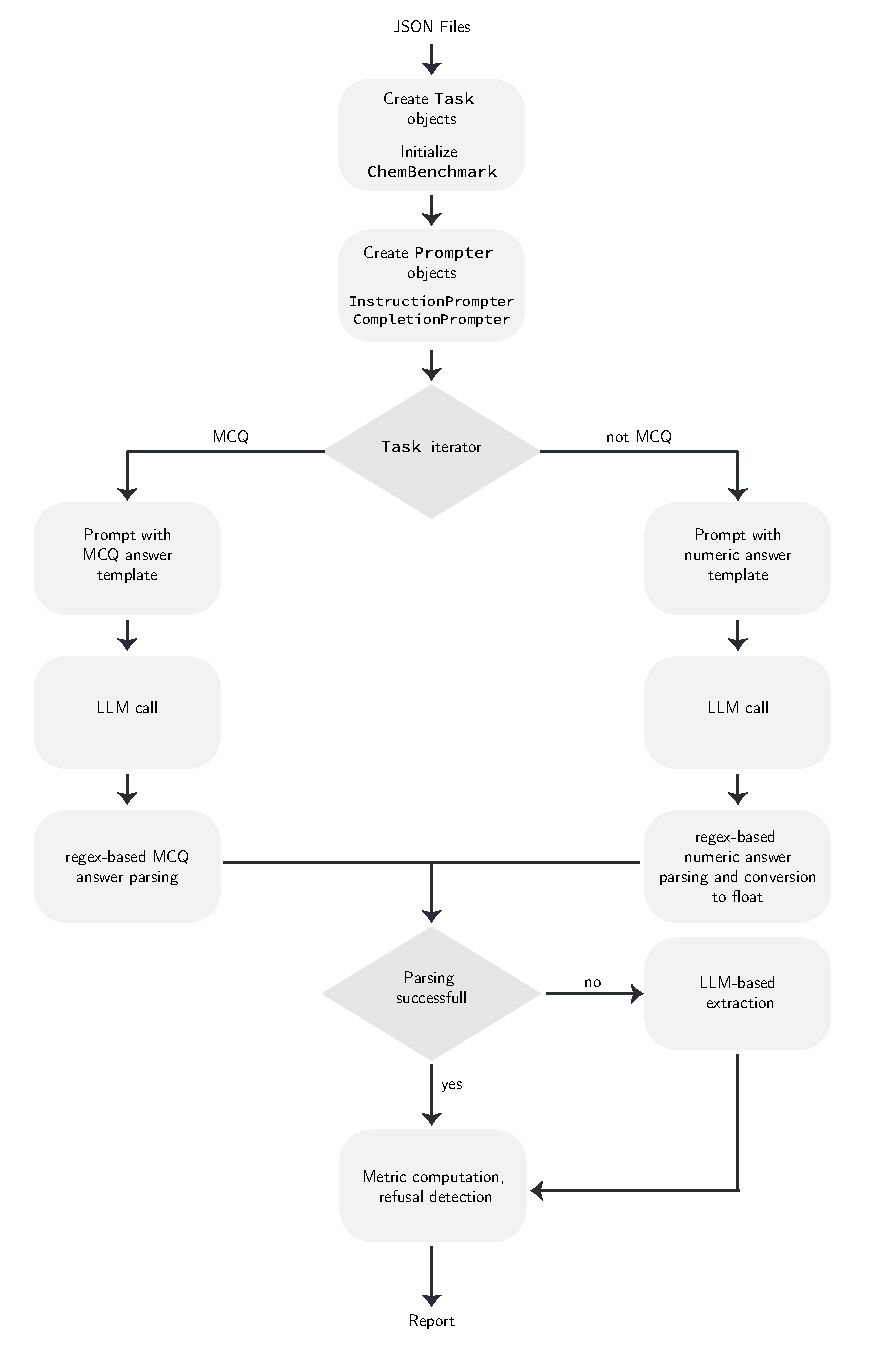
\includegraphics[height=.8\textheight]{figures/process.pdf}
    \caption{\textbf{Overview of the benchmarking pipeline implemented in \chembench.} The process begins with JSON files containing task data, which are used to create \texttt{Task} objects and initialize the \texttt{ChemBenchmark}. \texttt{Prompter} objects are then created to handle different types of prompts for instruction-tuned and completion models.
    The \texttt{Task} Iterator differentiates between \gls{mcq} and other question types. For each task type, appropriate prompts are generated and passed to the \gls{llm}. The responses are then processed using regex-based parsing methods specific to \gls{mcq} or numeric answers (after obtaining the relevant part of the response from the instruction-tuned models).
    The regex-based parsing is elaborate and also able to handle special cases such as scientific notation, or roman numerals.
    If the initial parsing is unsuccessful, the system employs an \gls{llm}-based extraction method as a fallback. The parsed or extracted answers then undergo metric computation and refusal detection.}
    \label{fig:process}
\end{figure}



\clearpage
\subsection{Human baseline} \label{sec:human_baseline}
\paragraph{App} To facilitate the collection of responses, we developed a responsive web application in Typescript using the Next.js\autocite{nextjs} app router framework.
This application handles serving the user interface and exposes various \gls{rest} \glspl{api} for relevant operations.
We utilize a Postgresql.
The web application is styled with Tailwind CSS\autocite{tailwindcss} using the shadcn/ui component library and uses NextAuth\autocite{nextauth} for easy and secure user authentication.
The application is hosted on the Vercel web hosting platform.

In the applications, human participants were presented with molecules as rendered drawings and SMILES strings. \LaTeX\xspace equations and chemical equations were rendered using MathJax\autocite{mathjax}.


\paragraph{Statistics}
\Cref{fig:human_score_distribution} shows the distribution of scores our human scorers achieved.

\begin{figure}[htb]
    \centering
    \includegraphics{figures/human_score_distribution.pdf}
    \script{plot_human_score_distribution.py}
    \caption{\textbf{Distribution of human scores.} The histogram and kernel density estimates show the fraction of questions answered completely correctly.
    Since the best possible score for each question is one and the worst possible score is zero, the values on this plot are between zero and one.}
    \label{fig:human_score_distribution}
\end{figure}

We also recorded the time humans took to answer the questions. This time is the time from the question being displayed to the human to the human submitting the answer.

\begin{figure}[htb]
    \centering
    \includegraphics{figures/human_timing.pdf}
    \script{analyze_human_data.py}
    \caption{\textbf{Time taken by human scorers to answer questions vs.\ correctness of their answers.} From the plot, it is clear that there is no clear dependence of the correctness of the answers on the time taken by the human scorers to answer the questions. However, we see that human scorers typically took longer to correctly answer questions with tool use.}
    \label{fig:human_timing}
\end{figure}

Additionally, we prompted users to provide additional information about their experience in chemistry.
While we recorded fine-grained information, e.g., their specialization, we focused on the number of years since the first university-level chemistry course.
\Cref{fig:experience_vs_correctness} shows that the experience of the human scorers was correlated with the correctness of their answers (\Cref{fig:experience_vs_correctness}, Spearman's \(\rho \approx \variable{output/spearman_experience_score.txt}\), and \(p \approx \variable{output/spearman_experience_score_p.txt}\)).

\begin{figure}[htb]
    \centering
    \includegraphics{figures/experience_vs_correctness.pdf}
    \script{analyze_human_data.py}
    \caption{\textbf{Experience of human  scorers vs.\ correctness of their answers.} The experience (in the number of years since the first university-level chemistry course) of the human scorers wasp correlated with the correctness of their answers.}
    \label{fig:experience_vs_correctness}
\end{figure}

\paragraph{Tool use}
In our study, humans were allowed to use tools for answering some questions.
They could also report what tools they used for answering questions. As \Cref{fig:tool_use} shows, the most commonly tool was some form of web search (which, according to the freetext responses, often was a multi-step process).

\clearpage
\subsection{Confidence estimates} \label{sec:confidence_estimates}

Since it is important to understand if models can provide an indication of whether their answer might likely be incorrect, we prompted some of our top performing \glspl{llm} to return the confidence in providing a correct answer on an ordinal scale.
This is similar to the verbalized confidence scores reported by \textcite{xiong2023llms}.
We find that the models show different distributions of confidence scores, which, for some, are skewed to the extremes.

In addition, we also analyzed the confidence estimated via the log probabilities of the answer tokens. This probability of a token given the context is not necessarily the same as the confidence in the correctness of the answer. However, it is still often used as a proxy.

Our analysis of both log probabilities and prompting confidence reveals distinct calibration behaviors across different language models.
\GPTFourO demonstrates an overconfident tendency, often assigning high probabilities even to incorrect answers.
However, when \GPTFourO displays high confidence, it accurately predicts correct answers approximately 80\% of the time. In contrast, \LlamaThreeOneEightBInstruct confidence distribution is more evenly spread, with a majority of predictions centered around 0.5. High-confidence predictions from \LlamaThreeOneEightBInstruct are less frequent compared to \GPTFourO, and unlike \GPTFourO, high confidence does not necessarily correlate with a higher chance of correct answers.
\begin{figure}[htb]
    \centering
    \includegraphics[width=\textwidth]{figures/log_probs_calibration_plot_overall_filtered.pdf}
    \caption{\textbf{Reliability diagram of histogram of logit-based confidence estimates.} For this analysis we obtained the linear probability from the logprobs of the models. Only logprobs of the tokens corresponding to the answers were considered. Linear proabability was computed by taking exponential of logprobs (for sequences with multiple tokens, values were multiplied).  The plot shows the average predicted probability and the fraction of correct answers for each bin of linear probabilities. The ideal scenario is a diagonal line, indicating perfect calibration where the model's confidence aligns perfectly with the actual correctness. The \gls{ece} value quantifies the overall calibration performance, with a lower \gls{ece} indicating better calibration.}
    \label{fig:confidence_score_distributions}
    \script{plot_logprobs.py}
\end{figure}

\clearpage
\subsection{Impact of sampling temperature}
We also investigated the impact of sampling temperature on the performance of the models. \Cref{fig:temperature_impact} shows that, generally, the performance of models tends to degrease with increasing temperature.

\begin{figure}
    \centering
    \includegraphics{figures/swarm_plot_combined.pdf}
    \caption{\textbf{Impact of sampling temperature on the performance of the models.} The plot shows the performance of the models at zero temperature (i.e., greedy decoding) and temperature of one. The performance is measured in terms of the fraction of questions answered correctly.}
    \label{fig:temperature_impact}
    \script{plot_temperature_diffs.py}
\end{figure}



\clearpage
\subsection{Leaderboard}
Our leaderboard is based on the tool chain developed for Matbench.\autocite{Dunn_2020}
Briefly, the \chembench pipeline produces standardized files in \texttt{json} format that contributors can add via pull requests to the \chembench repository.
The Markdown tables and interactive plots are automatically generated and updated on the \chembench website.

\clearpage

\printnoidxglossary[type=\acronymtype, nonumberlist]  % https://github.com/tectonic-typesetting/tectonic/issues/704
